\documentclass[11pt]{article}
\usepackage[margin=1in]{geometry}
\usepackage{amsmath, amssymb, amsthm}
\usepackage{booktabs}
\usepackage{graphicx}
\usepackage{hyperref}
\usepackage{cite}
\usepackage{tikz}
\usetikzlibrary{shapes, arrows, positioning, calc}
\usepackage{circuitikz}

\newtheorem{definition}{Definition}
\newtheorem{theorem}{Theorem}
\newtheorem{property}{Property}
\newtheorem{example}{Example}

\title{Pseudo-Random Binary Sequences for Ultrasonic Time-of-Flight Measurement: \\
\large A First-Principles Treatment of Correlation-Based Ranging}
\author{BATPING Project Technical Notes}
\date{June 2026}

\begin{document}
\maketitle

\begin{abstract}
This document provides a comprehensive, first-principles treatment of the theory underlying pseudo-random binary sequence (PRBS) waveforms for ultrasonic time-of-flight measurement. Beginning with the mathematical foundations of correlation and matched filtering, we develop the theory of linear feedback shift registers, maximum length sequences, Barker codes, and Golay complementary pairs. We then address the practical considerations of carrier modulation via binary phase-shift keying for narrowband piezoelectric transducers. Throughout, we emphasize the physical intuition behind each concept and its relevance to the BATPING acoustic thermometry system.
\end{abstract}

\tableofcontents
\newpage

%==============================================================================
\section{Introduction: The Time-of-Flight Problem}
%==============================================================================

\subsection{Physical Setup}

Consider an acoustic ranging system consisting of:
\begin{itemize}
    \item A transmitter that emits an acoustic waveform $x(t)$
    \item A propagation medium (air) with sound speed $c(T)$ depending on temperature
    \item A reflector at distance $d$ from the transducer
    \item A receiver (microphone) that records the reflected signal
\end{itemize}

The transmitted signal travels to the reflector and back, arriving at the receiver after a time delay:
\begin{equation}
\tau = \frac{2d}{c(T)}
\end{equation}

The speed of sound in air varies with temperature according to:
\begin{equation}
c(T) = 331.3\sqrt{1 + \frac{T}{273.15}} \approx 331.3 + 0.6T \quad \text{[m/s]}
\end{equation}

Inverting this relationship, temperature can be derived from the measured time-of-flight:
\begin{equation}
T = \frac{1}{0.6}\left(\frac{2d}{\tau} - 331.3\right)
\end{equation}

\subsection{The Precision Problem}

The fundamental challenge is that temperature precision depends directly on TOF precision:
\begin{equation}
\sigma_T = \left|\frac{\partial T}{\partial \tau}\right| \sigma_\tau = \frac{c^2}{0.6 \cdot 2d} \cdot \sigma_\tau
\end{equation}

For a 2-meter round-trip path at 20°C ($c \approx 343$ m/s):
\begin{equation}
\sigma_T \approx 98 \cdot \sigma_\tau \quad \text{[°C per second of TOF error]}
\end{equation}

To achieve 0.1°C precision, we need $\sigma_\tau < 1$ $\mu$s---a challenging requirement that motivates the search for optimal waveforms.

%==============================================================================
\section{Correlation: The Mathematical Foundation}
%==============================================================================

\subsection{Cross-Correlation Defined}

\begin{definition}[Cross-Correlation]
For two continuous signals $x(t)$ and $y(t)$, the cross-correlation function is:
\begin{equation}
R_{xy}(\tau) = \int_{-\infty}^{\infty} x(t) \cdot y(t + \tau) \, dt
\end{equation}
For discrete sequences $x[n]$ and $y[n]$ of length $N$:
\begin{equation}
R_{xy}[k] = \sum_{n=0}^{N-1-|k|} x[n] \cdot y[n + k]
\end{equation}
\end{definition}

The cross-correlation measures the similarity between $x$ and a time-shifted version of $y$. When $x = y$, this becomes the \textbf{autocorrelation}:
\begin{equation}
R_{xx}(\tau) = \int_{-\infty}^{\infty} x(t) \cdot x(t + \tau) \, dt
\end{equation}

\subsection{Physical Interpretation}

Consider sliding one signal past another and computing their inner product at each offset. The autocorrelation answers: ``How similar is a signal to delayed versions of itself?''

\begin{itemize}
    \item At $\tau = 0$: Perfect alignment, maximum value $R_{xx}(0) = \int |x(t)|^2 dt = E_x$ (signal energy)
    \item At $\tau \neq 0$: Measures self-similarity at that lag
\end{itemize}

For \textbf{ranging applications}, we transmit $x(t)$ and receive a delayed copy $r(t) = \alpha x(t - \tau_0) + n(t)$. The cross-correlation $R_{xr}(\tau)$ peaks at $\tau = \tau_0$, revealing the time delay.

\subsection{The Matched Filter}

\begin{theorem}[Matched Filter Optimality]
For detecting a known signal $x(t)$ in additive white Gaussian noise, the filter that maximizes the output signal-to-noise ratio is the \textbf{matched filter}:
\begin{equation}
h(t) = x^*(T - t)
\end{equation}
where $T$ is the signal duration and $^*$ denotes complex conjugation. For real signals, this simplifies to the time-reversed signal: $h(t) = x(T - t)$.
\end{theorem}

The matched filter output is precisely the cross-correlation:
\begin{equation}
y(t) = \int_{-\infty}^{\infty} r(\tau) \cdot h(t - \tau) \, d\tau = R_{xr}(t)
\end{equation}

This establishes correlation as the \textbf{optimal} detection strategy, not merely a convenient one.

\subsection{The Wiener-Khinchin Theorem}

\begin{theorem}[Wiener-Khinchin]
The autocorrelation function and power spectral density form a Fourier transform pair:
\begin{equation}
R_{xx}(\tau) \xleftrightarrow{\mathcal{F}} S_{xx}(f)
\end{equation}
\end{theorem}

This theorem has profound implications:
\begin{itemize}
    \item A signal with \textbf{flat (white) spectrum} has \textbf{impulsive autocorrelation}:
    \begin{equation}
    S_{xx}(f) = \text{constant} \quad \Longleftrightarrow \quad R_{xx}(\tau) = E \cdot \delta(\tau)
    \end{equation}
    \item The width of the autocorrelation main lobe is inversely proportional to bandwidth:
    \begin{equation}
    \Delta\tau \propto \frac{1}{B}
    \end{equation}
\end{itemize}

\textbf{Key insight:} To achieve a sharp correlation peak (precise ranging), we need a signal with wide, flat spectrum---i.e., a noise-like signal.

%==============================================================================
\section{The Ambiguity Function}
%==============================================================================

\subsection{Definition and Interpretation}

The autocorrelation considers only time shifts. In radar/sonar, moving targets also introduce Doppler shifts. The \textbf{ambiguity function} generalizes correlation to the delay-Doppler plane:

\begin{definition}[Narrowband Ambiguity Function]
\begin{equation}
\chi(\tau, f) = \int_{-\infty}^{\infty} x(t) \cdot x^*(t - \tau) \cdot e^{j2\pi f t} \, dt
\end{equation}
\end{definition}

At zero Doppler ($f = 0$), this reduces to the autocorrelation: $\chi(\tau, 0) = R_{xx}(\tau)$.

\subsection{Properties}

\begin{property}[Maximum at Origin]
\begin{equation}
|\chi(\tau, f)|^2 \leq |\chi(0, 0)|^2 = E^2
\end{equation}
The ambiguity function achieves its maximum at the origin.
\end{property}

\begin{property}[Volume Conservation]
\begin{equation}
\iint |\chi(\tau, f)|^2 \, d\tau \, df = E^2
\end{equation}
The total volume under $|\chi|^2$ is constant, regardless of waveform design.
\end{property}

This volume conservation implies a fundamental tradeoff: we cannot have arbitrarily sharp resolution in both range (delay) and velocity (Doppler) simultaneously. Energy concentrated near the origin in one dimension must spread in another.

\subsection{The Ideal ``Thumbtack'' Ambiguity Function}

The ideal ambiguity function would be:
\begin{equation}
\chi_{\text{ideal}}(\tau, f) = E \cdot \delta(\tau) \cdot \delta(f)
\end{equation}

This ``thumbtack'' function provides perfect resolution in both dimensions. However, it requires a signal with:
\begin{itemize}
    \item Infinite bandwidth (for $\delta(\tau)$)
    \item Infinite duration (for $\delta(f)$)
\end{itemize}

Such a signal would be ideal white noise---infinite energy, physically unrealizable. Nevertheless, we can \textbf{approximate} the thumbtack with noise-like signals of finite duration and bandwidth.

\subsection{Relevance to BATPING}

For acoustic thermometry, Doppler shifts are negligible (the air and reflector are stationary). We care primarily about the \textbf{zero-Doppler cut}---the autocorrelation $R_{xx}(\tau)$. Our goal is to minimize the width of the autocorrelation main lobe while suppressing sidelobes.

%==============================================================================
\section{Digital Logic Foundations}
%==============================================================================

Before introducing shift registers, we establish the necessary digital logic concepts.

\subsection{Binary Representation}

Digital systems represent information using two states: 0 and 1 (or equivalently, $-1$ and $+1$ for bipolar signaling). A \textbf{bit} is a single binary digit. A sequence of $n$ bits can represent $2^n$ distinct values.

\subsection{Logic Gates}

\begin{definition}[XOR Gate]
The exclusive-OR (XOR) operation, denoted $\oplus$, outputs 1 if and only if its inputs differ:
\begin{center}
\begin{tabular}{cc|c}
$A$ & $B$ & $A \oplus B$ \\
\midrule
0 & 0 & 0 \\
0 & 1 & 1 \\
1 & 0 & 1 \\
1 & 1 & 0 \\
\end{tabular}
\end{center}
\end{definition}

XOR is equivalent to modulo-2 addition: $A \oplus B = (A + B) \mod 2$.

\textbf{Properties of XOR:}
\begin{itemize}
    \item Commutative: $A \oplus B = B \oplus A$
    \item Associative: $(A \oplus B) \oplus C = A \oplus (B \oplus C)$
    \item Identity: $A \oplus 0 = A$
    \item Self-inverse: $A \oplus A = 0$
\end{itemize}

\subsection{Flip-Flops and Registers}

\begin{definition}[D Flip-Flop]
A D (data) flip-flop is a memory element that captures the input $D$ on each clock edge and holds it at output $Q$ until the next clock edge.
\end{definition}

\begin{center}
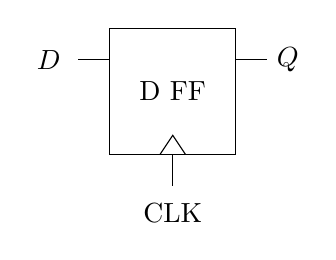
\begin{tikzpicture}[scale=0.8]
    \draw (0,0) rectangle (2,2);
    \node at (1,1) {D FF};
    \draw (-0.5,1.5) -- (0,1.5) node[left, xshift=-0.5cm] {$D$};
    \draw (2,1.5) -- (2.5,1.5) node[right] {$Q$};
    \draw (1,-0.5) -- (1,0) node[below, yshift=-0.5cm] {CLK};
    \draw (0.8,0) -- (1,0.3) -- (1.2,0);
\end{tikzpicture}
\end{center}

On each rising clock edge: $Q_{\text{new}} \leftarrow D$

\begin{definition}[Shift Register]
A shift register is a cascade of $n$ flip-flops where the output of each feeds the input of the next. On each clock cycle, data ``shifts'' through the chain.
\end{definition}

\begin{center}
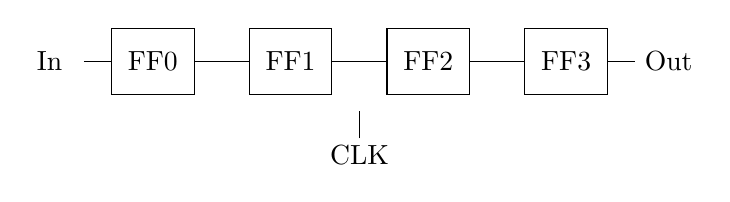
\begin{tikzpicture}[scale=0.7]
    % Flip-flops
    \foreach \i in {0,1,2,3} {
        \draw (\i*2.5,0) rectangle (\i*2.5+1.5,1.2);
        \node at (\i*2.5+0.75,0.6) {FF\i};
    }
    % Connections
    \draw (-0.5,0.6) -- (0,0.6) node[left, xshift=-0.5cm] {In};
    \draw (1.5,0.6) -- (2.5,0.6);
    \draw (4,0.6) -- (5,0.6);
    \draw (6.5,0.6) -- (7.5,0.6);
    \draw (9,0.6) -- (9.5,0.6) node[right] {Out};
    % Clock
    \draw (4.5,-0.8) -- (4.5,-0.3);
    \node at (4.5,-1.1) {CLK};
\end{tikzpicture}
\end{center}

A 4-bit shift register holds 4 bits. Each clock cycle:
\begin{itemize}
    \item A new bit enters from the left
    \item Each bit shifts one position right
    \item The rightmost bit exits
\end{itemize}

%==============================================================================
\section{Linear Feedback Shift Registers (LFSR)}
%==============================================================================

\subsection{Basic Structure}

A \textbf{Linear Feedback Shift Register} is a shift register whose input is a linear combination (XOR) of selected bit positions, called \textbf{taps}.

\begin{definition}[LFSR]
An $n$-stage LFSR consists of:
\begin{itemize}
    \item $n$ flip-flops holding state bits $s_0, s_1, \ldots, s_{n-1}$
    \item A feedback function: $s_{\text{new}} = c_1 s_0 \oplus c_2 s_1 \oplus \cdots \oplus c_n s_{n-1}$
    \item Coefficients $c_i \in \{0, 1\}$ defining which taps are active
\end{itemize}
\end{definition}

\begin{center}
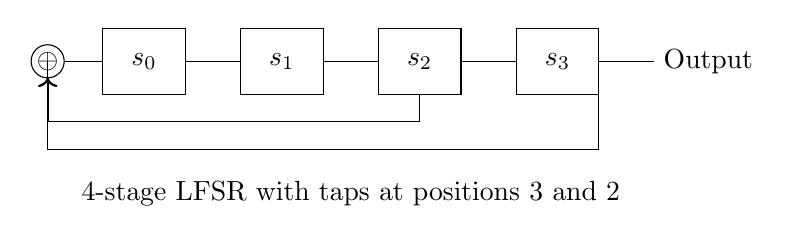
\begin{tikzpicture}[scale=0.7]
    % Flip-flops
    \foreach \i/\label in {0/$s_0$,1/$s_1$,2/$s_2$,3/$s_3$} {
        \draw (\i*2.5,0) rectangle (\i*2.5+1.5,1.2);
        \node at (\i*2.5+0.75,0.6) {\label};
    }
    % Forward connections
    \draw (1.5,0.6) -- (2.5,0.6);
    \draw (4,0.6) -- (5,0.6);
    \draw (6.5,0.6) -- (7.5,0.6);
    \draw (9,0.6) -- (10,0.6) node[right] {Output};

    % Feedback path
    \draw (9,0.6) -- (9,-1) -- (-1,-1) -- (-1,0.6);

    % XOR gate
    \draw (-1,0.6) circle (0.3);
    \node at (-1,0.6) {$\oplus$};
    \draw (-0.7,0.6) -- (0,0.6);

    % Tap from s_2
    \draw (5.75,0) -- (5.75,-0.5) -- (-1,-0.5);
    \draw[->, thick] (-1,-0.5) -- (-1,0.3);

    \node at (4.5,-1.8) {4-stage LFSR with taps at positions 3 and 2};
\end{tikzpicture}
\end{center}

\subsection{Fibonacci vs. Galois Configuration}

There are two equivalent LFSR architectures:

\textbf{Fibonacci LFSR:} Taps are XORed to produce the input to the first stage. The output is taken from the last stage.

\textbf{Galois LFSR:} Feedback is distributed---XOR gates are placed between stages. Often faster in hardware due to shorter combinational paths.

Both produce the same sequence (possibly with different phase).

\subsection{The Feedback Polynomial}

The LFSR is characterized by its \textbf{feedback polynomial} (also called characteristic polynomial):
\begin{equation}
p(x) = 1 + c_1 x + c_2 x^2 + \cdots + c_n x^n
\end{equation}
where $c_i = 1$ if tap $i$ is active.

\begin{example}
A 4-stage LFSR with taps at positions 4 and 3 (counting from 1) has polynomial:
\begin{equation}
p(x) = 1 + x^3 + x^4
\end{equation}
The feedback equation is: $s_{\text{new}} = s_3 \oplus s_4$ (using 1-based indexing).
\end{example}

\subsection{State Space and Periodicity}

An $n$-stage LFSR has $n$ bits of state, allowing $2^n$ possible states. However:
\begin{itemize}
    \item The all-zeros state $[0,0,\ldots,0]$ is \textbf{absorbing}---once entered, the LFSR stays there forever (since $0 \oplus 0 \oplus \cdots = 0$).
    \item The remaining $2^n - 1$ states form one or more cycles.
\end{itemize}

\begin{definition}[Primitive Polynomial]
A feedback polynomial is \textbf{primitive} if the LFSR cycles through all $2^n - 1$ non-zero states before repeating.
\end{definition}

With a primitive polynomial, starting from any non-zero state, the LFSR produces a sequence of period exactly $N = 2^n - 1$.

\subsection{Finding Primitive Polynomials}

Primitive polynomials exist for all $n$ and have been extensively tabulated. Some examples:

\begin{center}
\begin{tabular}{cll}
\toprule
$n$ & Primitive Polynomial & Period $N = 2^n - 1$ \\
\midrule
3 & $1 + x^2 + x^3$ & 7 \\
4 & $1 + x^3 + x^4$ & 15 \\
5 & $1 + x^3 + x^5$ & 31 \\
6 & $1 + x^5 + x^6$ & 63 \\
7 & $1 + x^6 + x^7$ & 127 \\
8 & $1 + x^2 + x^3 + x^4 + x^8$ & 255 \\
9 & $1 + x^5 + x^9$ & 511 \\
10 & $1 + x^7 + x^{10}$ & 1023 \\
\bottomrule
\end{tabular}
\end{center}

Two-tap (trinomial) primitive polynomials are preferred for simplicity when they exist.

%==============================================================================
\section{Maximum Length Sequences (m-sequences)}
%==============================================================================

\subsection{Definition}

\begin{definition}[Maximum Length Sequence]
A maximum length sequence (MLS or m-sequence) is the output of an LFSR with a primitive feedback polynomial. It has period $N = 2^n - 1$.
\end{definition}

For signal processing, we convert the binary $\{0, 1\}$ output to bipolar $\{-1, +1\}$:
\begin{equation}
a_k = 1 - 2 \cdot s_k = \begin{cases} +1 & \text{if } s_k = 0 \\ -1 & \text{if } s_k = 1 \end{cases}
\end{equation}

\subsection{Statistical Properties}

M-sequences have remarkable noise-like properties:

\begin{property}[Balance]
In one period, the sequence contains $(2^{n-1})$ ones and $(2^{n-1} - 1)$ zeros. The count differs by exactly 1.
\end{property}

\begin{property}[Run-Length Distribution]
A ``run'' is a consecutive sequence of identical bits. In one period:
\begin{itemize}
    \item Half of all runs have length 1
    \item One quarter have length 2
    \item One eighth have length 3
    \item And so on, with one run each of lengths $n-1$ and $n$
\end{itemize}
This mirrors the run distribution of a truly random binary sequence.
\end{property}

\begin{property}[Shift-and-Add]
The XOR of an m-sequence with any non-trivial cyclic shift of itself produces another cyclic shift:
\begin{equation}
a[k] \oplus a[k + m] = a[k + p] \quad \text{for some } p
\end{equation}
This is the defining property of m-sequences.
\end{property}

\subsection{Autocorrelation of M-Sequences}

\begin{theorem}[M-Sequence Autocorrelation]
The periodic autocorrelation of a bipolar m-sequence is:
\begin{equation}
R_{aa}[m] = \sum_{k=0}^{N-1} a_k \cdot a_{k+m \mod N} = \begin{cases}
N & m = 0 \mod N \\
-1 & m \neq 0 \mod N
\end{cases}
\end{equation}
\end{theorem}

This is remarkable: the autocorrelation is $N$ at zero lag and exactly $-1$ at all other lags. The sidelobe level relative to the peak is:
\begin{equation}
\text{Sidelobe level} = \frac{1}{N} \quad \Rightarrow \quad 20\log_{10}(N) \text{ dB below peak}
\end{equation}

\begin{center}
\begin{tabular}{ccc}
\toprule
$n$ & Sequence Length $N$ & Sidelobe Level \\
\midrule
5 & 31 & $-29.8$ dB \\
6 & 63 & $-36.0$ dB \\
7 & 127 & $-42.1$ dB \\
8 & 255 & $-48.1$ dB \\
9 & 511 & $-54.2$ dB \\
\bottomrule
\end{tabular}
\end{center}

\subsection{Power Spectrum}

The power spectrum of an m-sequence (viewed as periodic) consists of discrete spectral lines at harmonics of $1/N$ times the chip rate, with approximately equal amplitude---a nearly flat spectrum over the signal bandwidth.

For an aperiodic (single-period) m-sequence, the spectrum is continuous and approximately:
\begin{equation}
S(f) \approx T_c \cdot \text{sinc}^2(\pi f T_c)
\end{equation}
where $T_c$ is the chip duration. The main lobe extends to $f = 1/T_c$, giving bandwidth $B \approx 2/T_c$.

\subsection{Processing Gain}

\begin{definition}[Processing Gain]
The processing gain quantifies the SNR improvement from correlation:
\begin{equation}
G_p = \frac{\text{Peak correlation value}}{\text{RMS sidelobe level}} \approx N
\end{equation}
In decibels: $G_p[\text{dB}] = 10\log_{10}(N)$.
\end{definition}

For an $n$-stage LFSR producing a sequence of length $N = 2^n - 1$:
\begin{itemize}
    \item Peak value: $N$
    \item Sidelobe value: $-1$
    \item Processing gain: $N$ (or approximately $10 \cdot n \cdot \log_{10}(2) \approx 3n$ dB)
\end{itemize}

%==============================================================================
\section{Barker Codes}
%==============================================================================

\subsection{Definition and Optimality}

While m-sequences can be arbitrarily long, their sidelobes, though small relative to the peak, are all equal to $-1$. \textbf{Barker codes} achieve even better sidelobe performance for short sequences.

\begin{definition}[Barker Code]
A Barker code is a finite sequence $\{a_j\}_{j=1}^{N}$ with $a_j \in \{+1, -1\}$ such that the aperiodic autocorrelation satisfies:
\begin{equation}
|R_{aa}[k]| \leq 1 \quad \text{for all } k \neq 0
\end{equation}
\end{definition}

The constraint $|R[k]| \leq 1$ is the strongest possible---sidelobes are minimized to a single unit of correlation.

\subsection{All Known Barker Codes}

Remarkably, only \textbf{nine} Barker codes exist:

\begin{center}
\begin{tabular}{cll}
\toprule
Length $N$ & Code & Peak Sidelobe \\
\midrule
2 & $+1, -1$ (or $+1, +1$) & $-6.0$ dB \\
3 & $+1, +1, -1$ & $-9.5$ dB \\
4 & $+1, +1, -1, +1$ (or $+1, +1, +1, -1$) & $-12.0$ dB \\
5 & $+1, +1, +1, -1, +1$ & $-14.0$ dB \\
7 & $+1, +1, +1, -1, -1, +1, -1$ & $-16.9$ dB \\
11 & $+1, +1, +1, -1, -1, -1, +1, -1, -1, +1, -1$ & $-20.8$ dB \\
13 & $+1, +1, +1, +1, +1, -1, -1, +1, +1, -1, +1, -1, +1$ & $-22.3$ dB \\
\bottomrule
\end{tabular}
\end{center}

It has been proven that no odd-length Barker codes exist beyond length 13, and exhaustive computer search has found no even-length codes with $N < 10^{22}$.

\subsection{Autocorrelation Example: Barker-13}

For the length-13 Barker code $[+1, +1, +1, +1, +1, -1, -1, +1, +1, -1, +1, -1, +1]$:

\begin{center}
\begin{tabular}{c|cccccccccccccc}
Lag $k$ & 0 & 1 & 2 & 3 & 4 & 5 & 6 & 7 & 8 & 9 & 10 & 11 & 12 \\
\midrule
$R[k]$ & 13 & 0 & 1 & 0 & 1 & 0 & 1 & 0 & 1 & 0 & 1 & 0 & 1 \\
\end{tabular}
\end{center}

The peak is 13, sidelobes alternate between 0 and 1. The peak sidelobe level is $1/13 = -22.3$ dB.

\subsection{Comparison: Barker vs. MLS}

For short sequences ($N \leq 13$), Barker codes provide better sidelobe suppression than m-sequences of similar length:

\begin{center}
\begin{tabular}{l|cc|cc}
\toprule
& \multicolumn{2}{c|}{Barker} & \multicolumn{2}{c}{MLS} \\
$N$ & Available? & Sidelobe & Available? & Sidelobe \\
\midrule
7 & Yes & $-16.9$ dB & Yes ($n=3$) & $-16.9$ dB \\
13 & Yes & $-22.3$ dB & No & --- \\
15 & No & --- & Yes ($n=4$) & $-23.5$ dB \\
31 & No & --- & Yes ($n=5$) & $-29.8$ dB \\
\bottomrule
\end{tabular}
\end{center}

For longer sequences, MLS is the only option, and sidelobe levels improve with length.

%==============================================================================
\section{Golay Complementary Sequences}
%==============================================================================

\subsection{The Complementary Property}

\begin{definition}[Golay Complementary Pair]
Two sequences $A = \{a_k\}$ and $B = \{b_k\}$ of length $N$ form a Golay complementary pair if:
\begin{equation}
R_{AA}[k] + R_{BB}[k] = \begin{cases}
2N & k = 0 \\
0 & k \neq 0
\end{cases}
\end{equation}
\end{definition}

The key insight: while each sequence individually has non-zero sidelobes, these sidelobes \textbf{cancel exactly} when the autocorrelations are summed.

\subsection{Example: Length-4 Golay Pair}

Consider $A = [+1, +1, +1, -1]$ and $B = [+1, +1, -1, +1]$.

Autocorrelation of $A$:
\begin{align*}
R_{AA}[0] &= 1+1+1+1 = 4 \\
R_{AA}[1] &= 1+1-1 = 1 \\
R_{AA}[2] &= 1-1 = 0 \\
R_{AA}[3] &= -1
\end{align*}

Autocorrelation of $B$:
\begin{align*}
R_{BB}[0] &= 1+1+1+1 = 4 \\
R_{BB}[1] &= 1-1+1 = -1 \\
R_{BB}[2] &= -1+1 = 0 \\
R_{BB}[3] &= 1
\end{align*}

Sum:
\begin{align*}
R_{AA}[0] + R_{BB}[0] &= 4 + 4 = 8 = 2N \quad \checkmark \\
R_{AA}[1] + R_{BB}[1] &= 1 + (-1) = 0 \quad \checkmark \\
R_{AA}[2] + R_{BB}[2] &= 0 + 0 = 0 \quad \checkmark \\
R_{AA}[3] + R_{BB}[3] &= -1 + 1 = 0 \quad \checkmark
\end{align*}

\subsection{Construction Methods}

Golay pairs can be constructed recursively:

\textbf{Doubling construction:} Given a Golay pair $(A, B)$ of length $N$, construct a pair of length $2N$:
\begin{align}
A' &= [A, B] \\
B' &= [A, -B]
\end{align}
where $[X, Y]$ denotes concatenation.

Starting from the trivial pair $A = [1]$, $B = [1]$:
\begin{itemize}
    \item Length 2: $A = [1, 1]$, $B = [1, -1]$
    \item Length 4: $A = [1, 1, 1, -1]$, $B = [1, 1, -1, 1]$
    \item Length 8: $A = [1, 1, 1, -1, 1, 1, -1, 1]$, $B = [1, 1, 1, -1, -1, -1, 1, -1]$
\end{itemize}

This generates Golay pairs of length $2^m$. Other constructions yield lengths $10^j \cdot 26^k \cdot 2^m$.

\subsection{Practical Implementation}

To use Golay pairs for ranging:
\begin{enumerate}
    \item Transmit sequence $A$, receive and correlate with $A$, store result $R_A$
    \item Transmit sequence $B$, receive and correlate with $B$, store result $R_B$
    \item Compute $R_A + R_B$---sidelobes cancel, yielding a perfect impulse
\end{enumerate}

\textbf{Advantage:} Zero sidelobes (theoretically perfect autocorrelation).

\textbf{Disadvantage:} Requires two transmissions, doubling measurement time.

\subsection{Doppler Sensitivity}

A critical limitation of Golay pairs is \textbf{Doppler sensitivity}. The sidelobe cancellation relies on precise alignment of the two autocorrelations. Any Doppler shift between transmissions disrupts this alignment, reintroducing sidelobes.

Pezeshki et al.\ (2007) addressed this by ordering Golay pair transmissions according to the \textbf{Prouhet-Thue-Morse sequence}:
\begin{equation}
S = 0, 1, 1, 0, 1, 0, 0, 1, 1, 0, 0, 1, 0, 1, 1, 0, \ldots
\end{equation}
This sequence is constructed by: $s_0 = 0$, $s_{2k} = s_k$, $s_{2k+1} = 1 - s_k$.

Transmitting Golay pairs in PTM order annihilates low-order Taylor expansion terms of the composite ambiguity function, making it Doppler-resilient.

\textbf{For BATPING:} Doppler is negligible, so standard Golay pairs work without PTM ordering.

%==============================================================================
\section{Modulation: Baseband to Passband}
%==============================================================================

\subsection{The Narrowband Transducer Problem}

Our piezoelectric transducers are \textbf{resonant} devices with a narrow frequency response centered at 40 kHz. They cannot efficiently transmit:
\begin{itemize}
    \item DC or low-frequency signals
    \item Wideband baseband pulses
    \item Frequencies far from resonance
\end{itemize}

We must \textbf{modulate} our coded sequences onto a 40 kHz carrier to match the transducer's passband.

\subsection{Amplitude Modulation (AM)}

The simplest approach is amplitude modulation:
\begin{equation}
x(t) = a(t) \cdot \cos(2\pi f_c t)
\end{equation}
where $a(t)$ is the baseband signal and $f_c = 40$ kHz.

For a binary sequence, $a(t) \in \{0, 1\}$, this produces on-off keying (OOK). However, OOK is inefficient---half the time no energy is transmitted.

\subsection{Phase-Shift Keying (PSK)}

A more efficient approach encodes information in the \textbf{phase} of the carrier rather than its amplitude.

\begin{definition}[Binary Phase-Shift Keying (BPSK)]
In BPSK, the carrier phase takes one of two values (typically 0° and 180°) depending on the data bit:
\begin{equation}
x(t) = a_k \cdot \cos(2\pi f_c t) \quad \text{where } a_k \in \{+1, -1\}
\end{equation}
\end{definition}

Equivalently:
\begin{equation}
x(t) = \begin{cases}
+\cos(2\pi f_c t) & \text{if bit} = +1 \text{ (phase 0°)} \\
-\cos(2\pi f_c t) = \cos(2\pi f_c t + \pi) & \text{if bit} = -1 \text{ (phase 180°)}
\end{cases}
\end{equation}

\textbf{Key advantage:} The transmitter is always ``on''---constant envelope. This is important for:
\begin{itemize}
    \item Efficient use of amplifier (no clipping, operates in linear region)
    \item Maximum energy transfer to the transducer
    \item 3 dB SNR advantage over OOK at the receiver
\end{itemize}

\subsection{BPSK Waveform Construction}

For a code sequence $\{a_0, a_1, \ldots, a_{N-1}\}$ with chip duration $T_c$:
\begin{equation}
x(t) = \sum_{k=0}^{N-1} a_k \cdot p(t - kT_c) \cdot \cos(2\pi f_c t)
\end{equation}
where $p(t)$ is the \textbf{chip pulse shape}, typically:
\begin{itemize}
    \item Rectangular: $p(t) = 1$ for $0 \leq t < T_c$, else 0
    \item Raised cosine: Smoother transitions, reduced bandwidth
    \item Gaussian: $p(t) = \exp(-t^2/2\sigma^2)$, smooth with controlled bandwidth
\end{itemize}

\subsection{Spectrum of BPSK Signal}

For rectangular chip pulses, the baseband code has spectrum:
\begin{equation}
S_{\text{baseband}}(f) = T_c \cdot \text{sinc}^2(\pi f T_c)
\end{equation}

BPSK modulation shifts this to the carrier frequency:
\begin{equation}
S_{\text{BPSK}}(f) = \frac{T_c}{4}\left[\text{sinc}^2(\pi (f - f_c) T_c) + \text{sinc}^2(\pi (f + f_c) T_c)\right]
\end{equation}

The main lobe occupies $f_c \pm 1/T_c$. For our 40 kHz carrier:
\begin{itemize}
    \item $T_c = 100$ $\mu$s (10 kHz chip rate): Bandwidth spans 30--50 kHz
    \item $T_c = 200$ $\mu$s (5 kHz chip rate): Bandwidth spans 35--45 kHz
    \item $T_c = 250$ $\mu$s (4 kHz chip rate): Bandwidth spans 36--44 kHz
\end{itemize}

\subsection{Chip Rate and Carrier Cycles}

The relationship between chip duration and carrier cycles:
\begin{equation}
\text{Cycles per chip} = f_c \cdot T_c
\end{equation}

\begin{center}
\begin{tabular}{ccc}
\toprule
Chip Rate & $T_c$ & Cycles/Chip at 40 kHz \\
\midrule
10 kHz & 100 $\mu$s & 4 \\
8 kHz & 125 $\mu$s & 5 \\
5 kHz & 200 $\mu$s & 8 \\
4 kHz & 250 $\mu$s & 10 \\
\bottomrule
\end{tabular}
\end{center}

\textbf{Tradeoff:} More cycles per chip gives cleaner carrier (better for resonant transducers) but reduces bandwidth and hence range resolution.

\subsection{Phase Transitions}

At chip boundaries where $a_k \neq a_{k+1}$, the carrier phase flips by 180°. With rectangular pulses, this creates discontinuities. Options:
\begin{enumerate}
    \item \textbf{Accept discontinuities:} Simple, but causes spectral spreading and transducer ringing
    \item \textbf{Pulse shaping:} Use smooth pulse shapes (raised cosine, Gaussian) to reduce transitions
    \item \textbf{Minimum-shift keying:} Continuous phase modulation variant
\end{enumerate}

For narrowband transducers, discontinuities are somewhat filtered by the transducer itself, but pulse shaping improves performance.

%==============================================================================
\section{Pulse Shaping and Spectral Control}
%==============================================================================

\subsection{The Bandwidth-Resolution Tradeoff}

From the Wiener-Khinchin theorem:
\begin{equation}
\Delta\tau \cdot B \approx 1
\end{equation}

Wider bandwidth gives sharper correlation peaks. But:
\begin{itemize}
    \item Transducer bandwidth is limited ($\sim$10 kHz for our piezo)
    \item Out-of-band energy is wasted (not radiated efficiently)
    \item Spectral spreading can cause interference
\end{itemize}

Pulse shaping controls the spectrum while maintaining correlation properties.

\subsection{Common Pulse Shapes}

\textbf{Rectangular pulse:}
\begin{equation}
p(t) = \begin{cases} 1 & 0 \leq t < T_c \\ 0 & \text{otherwise} \end{cases}
\end{equation}
Spectrum: $P(f) = T_c \cdot \text{sinc}(\pi f T_c) \cdot e^{-j\pi f T_c}$

Sidelobes decay as $1/f$---slow rolloff, significant out-of-band energy.

\textbf{Raised cosine pulse:}
\begin{equation}
p(t) = \begin{cases}
\frac{1}{2}\left[1 - \cos\left(\frac{2\pi t}{T_c}\right)\right] & 0 \leq t < T_c \\
0 & \text{otherwise}
\end{cases}
\end{equation}
Smoother transitions, faster spectral rolloff.

\textbf{Gaussian pulse:}
\begin{equation}
p(t) = \exp\left(-\frac{(t - T_c/2)^2}{2\sigma^2}\right), \quad \sigma = \frac{T_c}{2\sqrt{2\ln 2}}
\end{equation}
The Gaussian is special: its Fourier transform is also Gaussian (the only function that is its own Fourier transform up to scaling). This gives optimal time-frequency concentration.

\subsection{Root Raised Cosine (RRC) Filtering}

In digital communications, \textbf{root raised cosine} filters are standard. The pulse shape is designed so that the cascade of transmit and matched filter gives a raised cosine response with zero intersymbol interference.

The RRC pulse with rolloff factor $\beta$ has spectrum:
\begin{equation}
P(f) = \begin{cases}
T_c & |f| \leq \frac{1-\beta}{2T_c} \\
T_c \cos^2\left(\frac{\pi T_c}{2\beta}\left(|f| - \frac{1-\beta}{2T_c}\right)\right) & \frac{1-\beta}{2T_c} < |f| \leq \frac{1+\beta}{2T_c} \\
0 & |f| > \frac{1+\beta}{2T_c}
\end{cases}
\end{equation}

\subsection{Effect on Autocorrelation}

Pulse shaping affects the correlation function. For BPSK with pulse shape $p(t)$:
\begin{equation}
R_{xx}(\tau) = R_{aa}[k] * R_{pp}(\tau - kT_c)
\end{equation}

where:
\begin{itemize}
    \item $R_{aa}[k]$ is the discrete code autocorrelation (Barker, MLS, etc.)
    \item $R_{pp}(\tau)$ is the continuous pulse autocorrelation
    \item $*$ denotes convolution
\end{itemize}

The pulse autocorrelation broadens the main lobe but also smooths sidelobes.

%==============================================================================
\section{Phase-Correlation Technique}
%==============================================================================

\subsection{Beyond Conventional Cross-Correlation}

Khyam et al.\ (2017) introduced a technique that achieves sharper TOF estimation than conventional cross-correlation without increasing physical bandwidth.

\textbf{Standard cross-correlation} in the frequency domain:
\begin{equation}
C(f) = S_T^*(f) \cdot S_R(f) = A_T(f) A_R(f) \cdot e^{j(\theta_R(f) - \theta_T(f))}
\end{equation}

Both amplitude and phase information are used. The inverse Fourier transform gives a peak at the time delay.

\textbf{Phase-correlation} discards amplitude information:
\begin{equation}
C_p(f) = e^{j(\theta_R(f) - \theta_T(f))}
\end{equation}

This sets all frequency components to unit magnitude, effectively ``whitening'' the spectrum.

\subsection{Mathematical Basis}

The inverse Fourier transform of a unit-magnitude, linear-phase signal is an impulse:
\begin{equation}
\mathcal{F}^{-1}\{e^{-j2\pi f \tau_0}\} = \delta(t - \tau_0)
\end{equation}

If the received signal is a delayed copy of the transmitted signal (no distortion), then:
\begin{equation}
\theta_R(f) - \theta_T(f) = -2\pi f \tau_0
\end{equation}

and phase-correlation yields:
\begin{equation}
c_p(t) = \mathcal{F}^{-1}\{C_p(f)\} = \delta(t - \tau_0)
\end{equation}

An \textbf{ideal impulse}---infinitely sharp.

\subsection{Practical Considerations}

In practice:
\begin{itemize}
    \item Noise corrupts the phase, especially outside the signal passband
    \item The signal has finite bandwidth (phase is meaningful only within the passband)
    \item Multipath creates multiple peaks
\end{itemize}

\textbf{Threshold-based detection:} Find the earliest peak above a threshold (typically 70\% of maximum) to identify the direct path in multipath conditions.

\textbf{SNR requirement:} Phase-correlation is more sensitive to noise. Khyam et al.\ found it effective for SNR $> 6$ dB. Below this, standard cross-correlation is more robust.

\subsection{Algorithm Summary}

\begin{enumerate}
    \item Compute FFT of transmitted signal: $S_T(f) = A_T(f) e^{j\theta_T(f)}$
    \item Compute FFT of received signal: $S_R(f) = A_R(f) e^{j\theta_R(f)}$
    \item Compute phase difference: $\Delta\theta(f) = \theta_R(f) - \theta_T(f)$
    \item Compute phase-correlation spectrum: $C_p(f) = e^{j\Delta\theta(f)}$
    \item Inverse FFT: $c_p(t) = \mathcal{F}^{-1}\{C_p(f)\}$
    \item Find maximum of $|c_p(t)|$ and apply threshold detection
\end{enumerate}

%==============================================================================
\section{Application to BATPING}
%==============================================================================

\subsection{System Constraints}

\begin{center}
\begin{tabular}{ll}
\toprule
Parameter & Value \\
\midrule
Carrier frequency & 40 kHz (piezo resonance) \\
Usable bandwidth & $\sim$10 kHz (35--45 kHz) \\
ADC sample rate & 384 kHz \\
AWG sample rate & 400 kHz \\
Repetition rate & 62.5 Hz \\
Path length & 2 m (round-trip) \\
Multipath delay & $\sim$5 ms (estimated) \\
\bottomrule
\end{tabular}
\end{center}

\subsection{Waveform Options}

\textbf{Option 1: Barker-13 BPSK}
\begin{itemize}
    \item 13 chips $\times$ 4 cycles/chip = 52 carrier cycles
    \item Duration: 52/40000 = 1.3 ms
    \item Chip rate: 10 kHz (bandwidth $\approx$ 10 kHz)
    \item Sidelobe level: $-22.3$ dB
    \item Processing gain: 11.1 dB
    \item Pros: Guaranteed low sidelobes, simple
    \item Cons: Limited length (only 13 chips available)
\end{itemize}

\textbf{Option 2: MLS-31 BPSK}
\begin{itemize}
    \item 31 chips (5-stage LFSR, polynomial $1 + x^3 + x^5$)
    \item Duration: 31 $\times$ 100 $\mu$s = 3.1 ms
    \item Sidelobe level: $-29.8$ dB
    \item Processing gain: 14.9 dB
    \item Pros: Higher gain than Barker
    \item Cons: Longer duration, closer to multipath limit
\end{itemize}

\textbf{Option 3: Golay Pair (Length 16)}
\begin{itemize}
    \item Two transmissions of 16 chips each
    \item Duration: 2 $\times$ 1.6 ms = 3.2 ms total
    \item Sidelobe level: 0 (theoretically perfect)
    \item Processing gain: 12 dB per transmission
    \item Pros: Zero sidelobes after summation
    \item Cons: Doubles measurement time
\end{itemize}

\subsection{Implementation Roadmap}

\begin{enumerate}
    \item \textbf{Characterize piezo response:} Measure actual frequency response and impulse response

    \item \textbf{Implement Barker-13:}
    \begin{itemize}
        \item Generate code: $[+1,+1,+1,+1,+1,-1,-1,+1,+1,-1,+1,-1,+1]$
        \item BPSK modulate onto 40 kHz carrier with Gaussian pulse shaping
        \item Upload to SDG1062X
        \item Record response, compute correlation, measure peak width
    \end{itemize}

    \item \textbf{Implement MLS-31:}
    \begin{itemize}
        \item Generate sequence using 5-stage LFSR
        \item Same modulation and testing procedure
        \item Compare SNR and sidelobe levels to Barker-13
    \end{itemize}

    \item \textbf{Test Golay pairs:}
    \begin{itemize}
        \item Generate length-16 pair using doubling construction
        \item Implement two-transmission protocol
        \item Verify sidelobe cancellation
    \end{itemize}

    \item \textbf{Apply phase-correlation:}
    \begin{itemize}
        \item Implement Khyam's algorithm on recorded data
        \item Compare peak sharpness with standard correlation
        \item Determine SNR threshold for reliable operation
    \end{itemize}
\end{enumerate}

\subsection{Expected Performance}

Based on the 10 kHz bandwidth limit:
\begin{equation}
\Delta\tau_{\min} \approx \frac{1}{B} = \frac{1}{10\text{ kHz}} = 100 \text{ }\mu\text{s}
\end{equation}

This corresponds to:
\begin{equation}
\Delta d = c \cdot \Delta\tau = 343 \times 100 \times 10^{-6} = 3.4 \text{ cm range resolution}
\end{equation}

Temperature precision (for 2 m path):
\begin{equation}
\sigma_T = \frac{c^2}{0.6 \cdot d} \cdot \sigma_\tau = \frac{343^2}{0.6 \cdot 2} \cdot 100 \times 10^{-6} \approx 9.8 \text{ °C}
\end{equation}

This seems large, but:
\begin{itemize}
    \item Processing gain improves SNR, enabling sub-sample peak localization
    \item Averaging multiple measurements reduces variance
    \item Phase-correlation can sharpen the peak beyond the bandwidth limit
\end{itemize}

With matched filtering and proper peak interpolation, sub-microsecond precision is achievable, corresponding to sub-0.1°C temperature precision.

%==============================================================================
\section{Summary}
%==============================================================================

This document has developed the theoretical framework for PRBS-based TOF measurement:

\begin{enumerate}
    \item \textbf{Correlation} is the optimal detection strategy for known signals in noise. The autocorrelation function determines ranging precision.

    \item \textbf{The Wiener-Khinchin theorem} connects autocorrelation to spectrum: flat spectrum $\Leftrightarrow$ impulsive autocorrelation.

    \item \textbf{LFSRs} with primitive polynomials generate maximum length sequences---the longest possible periodic sequences from $n$ bits of state.

    \item \textbf{M-sequences} have near-ideal autocorrelation: peak of $N$, constant sidelobes of $-1$. Processing gain scales with sequence length.

    \item \textbf{Barker codes} achieve optimal sidelobe suppression for short sequences ($N \leq 13$). Only nine exist.

    \item \textbf{Golay pairs} provide theoretically perfect autocorrelation (zero sidelobes) at the cost of two transmissions.

    \item \textbf{BPSK modulation} maps binary codes onto a carrier suitable for narrowband transducers. The chip rate determines bandwidth.

    \item \textbf{Pulse shaping} controls spectral characteristics and affects the correlation function.

    \item \textbf{Phase-correlation} can achieve sharper peaks than standard correlation by effectively whitening the spectrum, at the cost of noise sensitivity.
\end{enumerate}

For the BATPING system, the recommended approach is:
\begin{itemize}
    \item Start with Barker-13 BPSK as a robust baseline
    \item Progress to MLS-31 for improved processing gain
    \item Consider Golay pairs if sidelobes remain problematic
    \item Apply phase-correlation for final precision improvement
\end{itemize}

%==============================================================================
\section{References}
%==============================================================================

\begin{enumerate}
    \item Golay, M.J.E. (1961). ``Complementary series.'' \textit{IRE Trans. Inform. Theory}, 7(2):82--87.

    \item Barker, R.H. (1953). ``Group synchronization of binary digital systems.'' \textit{Communication Theory}, pp. 273--287.

    \item Khyam, M.O., et al. (2017). ``Highly accurate time-of-flight measurement technique based on phase-correlation for ultrasonic ranging.'' \textit{IEEE Sensors Journal}, 17(2):434--443.

    \item Pezeshki, A., et al. (2007). ``Doppler resilient Golay complementary pairs for radar.'' \textit{Proc. IEEE SSP Workshop}.

    \item Allen, K.C. and Lindsay-Stewart, W.A. (1994). ``Method and apparatus for measuring the impulse response of a radio channel.'' US Patent 5,371,760.

    \item Misaridis, T. and Jensen, J.A. (2005). ``Use of modulated excitation signals in medical ultrasound.'' \textit{Ultrasonics}, 43:668--690.

    \item Golomb, S.W. (1967). \textit{Shift Register Sequences}. Holden-Day.

    \item Proakis, J.G. and Salehi, M. (2008). \textit{Digital Communications}, 5th ed. McGraw-Hill.
\end{enumerate}

\end{document}
